\documentclass[11pt,a4paper]{article}

% Packages
\usepackage[margin=2.4cm]{geometry}
\usepackage{hyperref}
\usepackage{booktabs}
\usepackage{enumitem}
\usepackage{titlesec}
\usepackage{fancyhdr}
\usepackage{setspace}
\usepackage{graphicx}
\usepackage{xcolor}
\usepackage{amsmath}
\usepackage{amssymb}
\usepackage{longtable}
\usepackage{array}
\usepackage{url}
\usepackage{parskip}
\usepackage{tikz}
\usepackage{tcolorbox}
\usepackage{tabularx}
\usepackage{multirow}
\usepackage{colortbl}
\usepackage{float}

\usetikzlibrary{shapes.geometric,arrows.meta,positioning,fit,calc,backgrounds}

% Hyperref
\hypersetup{
    colorlinks=true,
    linkcolor=blue!60!black,
    citecolor=blue!60!black,
    urlcolor=blue!60!black
}

% Title formats
\titleformat{\section}{\large\bfseries}{\thesection}{1em}{}
\titleformat{\subsection}{\normalsize\bfseries}{\thesubsection}{1em}{}
\titleformat{\subsubsection}{\normalsize\itshape}{\thesubsubsection}{1em}{}

% Header/Footer
\pagestyle{fancy}
\fancyhf{}
\fancyhead[L]{\small Distributed Fiduciary Governance Model}
\fancyhead[R]{\small Expanded Policy Paper}
\fancyfoot[C]{\thepage}
\renewcommand{\headrulewidth}{0.4pt}

\onehalfspacing

% Colours
\definecolor{modelblue}{RGB}{30,70,120}
\definecolor{modelgreen}{RGB}{40,120,80}
\definecolor{modelorange}{RGB}{180,90,30}
\definecolor{modelgray}{RGB}{90,90,90}
\definecolor{lightblue}{RGB}{230,240,250}
\definecolor{lightgreen}{RGB}{230,245,235}
\definecolor{lightorange}{RGB}{255,240,220}

% Boxes
\tcbuselibrary{skins,breakable}
\newtcolorbox{principlebox}[1][]{
    colback=lightblue,colframe=modelblue,fonttitle=\bfseries,
    title=#1,breakable,left=4pt,right=4pt,top=3pt,bottom=3pt
}
\newtcolorbox{warningbox}[1][]{
    colback=lightorange,colframe=modelorange,fonttitle=\bfseries,
    title=#1,breakable,left=4pt,right=4pt,top=3pt,bottom=3pt
}
\newtcolorbox{modulebox}[1][]{
    colback=lightgreen,colframe=modelgreen,fonttitle=\bfseries,
    title=#1,breakable,left=4pt,right=4pt,top=3pt,bottom=3pt
}

\title{
\textbf{Redesigning Democratic Accountability}\\[0.3em]
\large Incentive Inversion, Near-Term Integrity Reform,\\
and Experimental Pathways for Australia
}
\author{
Policy Discussion Paper\\[0.4em]
\textit{Working Draft --- Version 3}
}
\date{August 2026}

\begin{document}

\maketitle


\begin{abstract}
\noindent
Australia’s arrangements for political access, formal advice, and post-office employment systematically favour private influence over public audit. The \textbf{basic idea} of this paper is simple: \emph{invert the incentive structure} so that closed-door influence becomes higher-cost and lower-return, while public scrutiny becomes cheaper and more complete.

The actionable core is a near-term integrity package---mandatory ministerial diaries, a functionally defined influence register, enforceable cooling-off with disclosure, selected public advice records, and independent oversight---that can be legislated without constitutional redesign. These measures map onto agendas already advanced by integrity-focused parliamentarians and have comparative precedents.

Beyond that core, the paper sketches \textbf{potential improvements} that might further improve democratic accountability and long-horizon public decision-making: preferential citizen signalling, competency-aware selection aids, region-first competence pilots, and related architecture. Those extensions are explicitly \emph{experimental}. They are not presented as settled institutional truth. Each is accompanied by a pilot design, pre-registered success metrics, and falsification criteria, because claims about a ``better running society'' require empirical evidence before scale-up.

Version~3 therefore separates (A)~what should be done now on existing evidence and integrity practice from (B)~what should be tested carefully before being treated as architecture.
\end{abstract}

\tableofcontents
\newpage

\section{Introduction and Problem Diagnosis}

Democratic legitimacy depends on the capacity of citizens and intermediary institutions to observe, contest, and correct public power. When influence channels are opaque, post-separation employment rules are weakly enforced, and formal advice remains largely private, practical accountability erodes even while elections continue.

Australian federal practice displays several reinforcing features:

\begin{itemize}[leftmargin=*]
    \item Ministerial diaries and meeting records are not subject to a strong, uniform, timely public disclosure regime.
    \item The formal lobbyist register captures only a minority of professional influence activity; in-house government-relations work and many forms of sponsored parliamentary access remain outside effective public view.
    \item Cooling-off and post-separation employment rules for ministers and senior officials have repeatedly proven porous.
    \item Advisory and consultancy ecosystems create recurring pathways for industry-aligned expertise to shape policy while underlying interests and prior relationships stay imperfectly visible.
\end{itemize}

These are not primarily failures of individual character. They are predictable products of institutional design that makes private access relatively cheap and public scrutiny relatively costly. Organised interests can systematically out-compete diffuse public interests in the contest for ministerial time and policy attention.

\begin{principlebox}{Core diagnosis}
The central design failure is an inverted incentive structure: closed-door influence is high-return and low-visibility; public audit is high-cost and incomplete. Any durable remedy must invert those relative returns.
\end{principlebox}

This paper does not treat lobbying or expertise as illegitimate. It argues that the \textit{terms} on which influence and advice operate must be rebalanced toward transparency, verifiable independence of formal advisors, and structural reduction in the decisive power of private channels.

\section{The Basic Idea}

\begin{principlebox}{One sentence}
Raise the cost and visibility of privileged private access; lower the cost of public audit of advice and influence trails.
\end{principlebox}

Operationally, that means five near-term instruments that reinforce one another:

\begin{enumerate}[leftmargin=*]
    \item \textbf{Publish access.} Mandatory, timely, machine-readable ministerial (and senior-official) diaries.
    \item \textbf{Widen the register.} Functional coverage of influence activity, including in-house and sponsored access---not a narrow ``lobbyist'' occupational label.
    \item \textbf{Enforce separation.} Longer cooling-off, real sanctions, public post-separation employment disclosure, anti-avoidance rules.
    \item \textbf{Open selected advice.} Public records (summaries or transcripts) for defined high-impact decision categories, with narrow reviewable exceptions.
    \item \textbf{Resource oversight.} Independent capacity to monitor compliance and report publicly.
\end{enumerate}

That package \emph{is} the paper’s policy claim. Everything else in this draft is either (i)~supporting comparative context, (ii)~risk analysis for implementing the package, or (iii)~an experimental agenda for reforms that \emph{might} improve governance further but are not yet evidenced at Australian scale.

\begin{warningbox}{What this paper is not claiming}
Region-first legal hierarchy, competency-scored entry to political roles, and preferential citizen signalling over public expenditure are \textbf{not} presented here as ready-to-enact national architecture. They are candidate improvements whose social value is an empirical question. Without pilots, pre-registered metrics, and honest failure criteria, they risk becoming technocratic fashion rather than democratic reform.
\end{warningbox}

\section{Design Principles for the Near-Term Package}

The near-term package rests on four interlocking principles. (Two further principles---region-first subsidiarity and competency as a visible selection criterion---are deferred to the experimental section because they are not required to deliver the basic idea.)

\begin{enumerate}[leftmargin=*]
    \item \textbf{Transparency by default.} Formal advice and records of significant access are public unless a narrowly defined, independently reviewable exception applies.
    \item \textbf{Reduced returns to private access.} Rules should make closed-door influence less decisive relative to open, documented, contestable processes.
    \item \textbf{Anti-capture constraints.} Employment, placement, and disclosure rules actively impede revolving-door and proxy capture of advisory functions.
    \item \textbf{Long-horizon institutional duty (bounded).} Oversight and selected advisory bodies should carry explicit obligations to report on intergenerational and systemic effects that ordinary electoral cycles undervalue---without displacing ministerial responsibility to Parliament.
\end{enumerate}

Transparency without anti-capture can be gamed by volume. Anti-capture without transparency can hide in informal channels. The package therefore treats them as complements.

\section{Glossary of Key Concepts}

\noindent
Terms below are defined as used in this paper. Ordinary political-science meanings apply unless noted. Paper-specific or specialised senses are marked.

\begin{description}[style=nextline,leftmargin=1.4em,font=\normalfont\bfseries]

\item[Adaptive re-capture]
Lawful workarounds after an integrity reform that restore privileged access (new intermediaries, timing games, forum-shifting). Expected residual risk; requires anti-avoidance drafting and continuous review.

\item[Anti-capture constraints]
Employment, placement, cooling-off, and disclosure rules that impede revolving-door and proxy capture of advisory functions---changing structural returns, not merely labelling conflicts.

\item[Anti-brigading design]
Participatory safeguards limiting coordinated mobilisation that would skew signalling or open-issue systems toward well-resourced groups.

\item[Basic idea (incentive inversion)]
Institutional redesign that raises the cost/visibility of privileged private access and lowers the cost of public audit of advice and influence trails.

\item[Competency-aware selection \emph{(experimental)}]
Supplementary capability demonstrations (open simulations, prior-performance records, scored program assessment) used alongside electoral or appointment legitimacy. Not a replacement for elections; not endorsed for scale-up without pilot evidence.

\item[Cooling-off period]
Statutory interval after leaving office during which specified private employment, lobbying, or advisory activity is restricted, with enforceable duration, sanctions, and public post-separation registers.

\item[Experimental track]
A proposed reform treated as a testable hypothesis: implemented only in limited pilots, with pre-registered metrics, comparison conditions, and explicit stop/adapt/scale rules.

\item[Functional coverage of influence activity]
Register design capturing influence by what actors do---including in-house government-relations and sponsored access---rather than by a narrow ``lobbyist'' label.

\item[Inverted incentive structure]
Settings where closed-door influence is high-return and low-visibility, while public audit is high-cost and incomplete.

\item[Near-term integrity package]
The actionable core of this paper: diaries, expanded influence register, enforceable cooling-off, selected public advice records, and independent oversight.

\item[Preferential citizen signalling \emph{(experimental)}]
Structured citizen preference input over a defined discretionary spending envelope under equal weighting and campaign transparency. Advisory unless a pilot protocol expressly tests binding rules.

\item[Proxy capture]
Indirect capture via consultancies, secondees, revolving placements, or aligned ``independent'' experts.

\item[Region-first competence \emph{(experimental)}]
Allocating primary operational competence for suitably scaled matters to regional bodies, subject to residual national functions. In Australia this is a pilot hypothesis within existing multi-level government, not a presumption of constitutional redesign.

\item[Residual national functions]
Network-level powers for non-separable or large-externality domains (defence, monetary integrity, major inter-regional infrastructure, baseline rights/equity floors, treaty implementation).

\item[Transition capture]
Intensified influence activity between announcement and enforcement of new rules.

\item[Transparency by default]
Presumption that formal advice and significant access records are public, with narrow, reviewable, preferably time-limited exceptions.

\end{description}

\section{The Near-Term Integrity Package}

\subsection{Module specifications}

\begin{modulebox}{Module 1 --- Mandatory Ministerial Diaries}
Legislation or binding standards requiring publication within 14--28 days; machine-readable format; limited enumerated exceptions; independent review; delayed-release schedules; annual public statistics on exception rates.
\end{modulebox}

\begin{modulebox}{Module 2 --- Expanded Influence Register}
Functional definition of registrable influence activity covering in-house and sponsored access. Public, searchable, timely register with meaningful penalties.
\end{modulebox}

\begin{modulebox}{Module 3 --- Enforced Cooling-Off + Disclosure}
Longer statutory periods, real sanctions, public register of relevant post-separation employment, independent monitoring, and anti-avoidance rules.
\end{modulebox}

\begin{modulebox}{Module 4 --- Public Advice Records (Selected Categories)}
Start with a defined list of high-impact decisions. Structured summaries or transcripts by default. Narrow exceptions with review.
\end{modulebox}

\begin{modulebox}{Module 5 --- Independent Oversight Capacity}
Resourced monitoring of compliance across Modules 1--4, public reporting, and authority to refer non-compliance for sanction.
\end{modulebox}

\begin{modulebox}{Module 6 --- Open Issue / Complaint Platform (optional near-term)}
Categorised public system with private security channel, published escalation thresholds, independent oversight, and durable archive. Can proceed with the package or as a linked pilot.
\end{modulebox}

\subsection{Mapping to documented weaknesses}

\begin{table}[H]
\centering
\small
\begin{tabular}{@{}p{4.0cm}p{5.2cm}p{4.3cm}@{}}
\toprule
\textbf{Current weakness} & \textbf{Model response} & \textbf{Near-term instrument} \\
\midrule
No strong diary publication & Transparency default for meetings & Mandatory timely diary publication \\
Narrow lobbyist definition & Functional coverage of influence activity & Expanded register \& code \\
Porous revolving door & Employment \& cooling-off constraints & Longer enforced cooling-off + disclosure \\
Private formal advice & Public advice records by default & Selected-category advice publication \\
Weak monitoring & Independent compliance capacity & Oversight body with public reporting \\
\bottomrule
\end{tabular}
\caption{Mapping of documented influence problems to the near-term package.}
\label{tab:lobbyingmap}
\end{table}

\subsection{Implementation friction (near-term)}

\begin{itemize}[leftmargin=*]
    \item Strong resistance to diary publication and exception discipline.
    \item Public-service and consultancy opposition to cooling-off rules.
    \item Potential chilling of frank advice (mitigate with structured summaries and delayed release).
    \item Transition windows for intensified influence activity (mitigate with rapid commencement and anti-avoidance language).
    \item Administrative under-capacity if oversight is announced without funding.
\end{itemize}

\section{Comparative Integrity Context}

The near-term package is not invented from a blank page. Comparable instruments exist, with uneven results that should discipline Australian design:

\begin{description}[style=nextline,leftmargin=1.2em]
    \item[Ministerial diaries / access transparency.]
    Jurisdictions that publish ministerial meetings on fixed timetables show that routine disclosure is administratively feasible. Design quality turns on exception breadth, machine-readability, and whether non-compliance carries consequences. Australia’s gap is less conceptual than enforcement and uniformity.

    \item[Lobbying / influence registers.]
    Canadian and related regimes illustrate both the value and the failure mode of registers: if coverage tracks occupational labels rather than influence \emph{activity}, in-house and sponsored channels remain dark. Functional definitions and penalties matter more than the existence of a list.

    \item[Cooling-off / post-separation rules.]
    Many systems announce cooling-off periods that are short, waivable, or weakly monitored. Comparative lesson: duration without monitoring and anti-avoidance is largely symbolic.

    \item[Advice and decision records.]
    Freedom-of-information and proactive release regimes (including stronger proactive cultures in some Westminster peers) show that selected high-impact advice can be published without collapsing cabinet government---if categories, delays, and review are tightly specified.
\end{description}

\begin{principlebox}{Inference for Australia}
Enough comparative practice exists to justify legislating the near-term package now. Comparative practice does \emph{not} yet justify national rollout of competency-scored political selection, expenditure signalling as a standing fourth chamber, or a new regional tier. Those require Australian pilots.
\end{principlebox}

\section{Potential Improvements That Need Empirical Evidence}

The fuller architecture explored in earlier drafts---region-first hierarchy, competency mechanisms, preferential signalling, long-horizon fiduciary bodies---may improve democratic accountability and social decision quality. Or it may introduce technocratic bias, participation skew, coordination failure, or new capture surfaces.

Version~3 therefore demotes those ideas to \textbf{experimental tracks}. Each track states a hypothesis, a bounded pilot, primary metrics, and stop/adapt/scale rules. No track is a commitment to national architecture.

\begin{figure}[H]
\centering
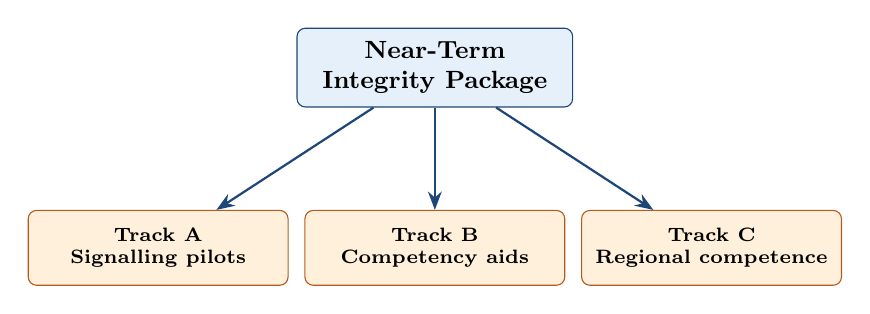
\begin{tikzpicture}[
    node distance=0.7cm and 0.9cm,
    box/.style={rectangle, draw=modelblue, fill=lightblue, rounded corners=3pt,
                minimum width=3.5cm, minimum height=1.0cm, align=center, font=\small\bfseries},
    exp/.style={rectangle, draw=modelorange, fill=lightorange, rounded corners=3pt,
                minimum width=3.3cm, minimum height=0.95cm, align=center, font=\scriptsize\bfseries},
    arrow/.style={-{Stealth}, thick, modelblue}
]
\node[box] (core) {Near-Term\\Integrity Package};
\node[exp, below left=1.3cm and 0.1cm of core] (e1) {Track A\\Signalling pilots};
\node[exp, below=1.3cm of core] (e2) {Track B\\Competency aids};
\node[exp, below right=1.3cm and 0.1cm of core] (e3) {Track C\\Regional competence};
\draw[arrow] (core) -- (e1);
\draw[arrow] (core) -- (e2);
\draw[arrow] (core) -- (e3);
\end{tikzpicture}
\caption{Policy core versus experimental tracks. Scale-up of orange nodes requires evidence.}
\label{fig:core-vs-experiment}
\end{figure}

\subsection{Experimental Track A --- Preferential Citizen Signalling}

\paragraph{Hypothesis.}
Equal-weighted citizen signalling over a small discretionary expenditure envelope improves perceived legitimacy and allocative alignment relative to opaque ministerial discretion, without catastrophic brigading or capture by organised campaigns.

\paragraph{Pilot design.}
\begin{itemize}[leftmargin=*]
    \item \textbf{Sites:} 2--3 local government areas or a single state discretionary grants program; duration 12--18 months.
    \item \textbf{Treatment:} A defined envelope (e.g.\ 1--3\% of discretionary spend) subject to preferential signalling; protected baselines excluded; full transparency of results and organised campaigns; anti-brigading rules published in advance.
    \item \textbf{Comparison:} Matched untreated programs, or stepped-wedge rollout across sites.
    \item \textbf{Unit of analysis:} Projects/grants and participating citizens; pre-registered analysis plan.
\end{itemize}

\paragraph{Primary metrics.}
Participation rate and demographic representativeness; concentration of influence (Herfindahl of campaign-linked signals); share of envelope captured by organised campaigns; post-decision legitimacy surveys; administrative cost per dollar allocated; time-to-decision.

\paragraph{Stop / adapt / scale rules.}
Stop or redesign if participation is severely skewed, campaign capture exceeds a pre-set threshold, or legitimacy falls relative to comparison sites. Scale only after independent evaluation and legislative review---not by administrative creep.

\subsection{Experimental Track B --- Competency-Aware Selection Aids}

\paragraph{Hypothesis.}
Open, audited capability demonstrations for \emph{selected appointed} roles (not general elections) improve candidate quality and public confidence without entrenching cultural or socio-economic bias.

\paragraph{Pilot design.}
\begin{itemize}[leftmargin=*]
    \item \textbf{Scope limit:} Appointed boards, statutory offices, or senior advisory panels---\emph{not} parliamentary candidacy in the first pilots.
    \item \textbf{Sites:} 2--4 appointment processes over 24 months.
    \item \textbf{Treatment:} Open-source or fully documented scenarios; version control; published scoring frameworks; structural separation of scenario designers from appointing authorities; parallel qualitative evaluation; bias audit.
    \item \textbf{Comparison:} Parallel conventional shortlisting on matched roles, or before/after process audits with blinded external review of appointee dossiers.
\end{itemize}

\paragraph{Primary metrics.}
Inter-rater reliability of scores; bias audit outcomes (demographic and experiential); correlation (if any) with subsequent performance indicators agreed ex ante; public confidence measures; rate of successful legal/process challenge; coaching/gaming incident reports.

\paragraph{Stop / adapt / scale rules.}
Do not extend to elective office unless appointed-role pilots clear bias and legitimacy thresholds. Any electoral use would be a separate, higher-bar experiment with explicit democratic safeguards and parliamentary consent.

\begin{warningbox}{Democratic boundary}
Elections remain central. Competency tools that gate \emph{who may stand} are a different---and far more contentious---institution than tools that inform \emph{whom a minister appoints}. Track~B starts only with the latter.
\end{warningbox}

\subsection{Experimental Track C --- Region-First Competence Pilots}

\paragraph{Hypothesis.}
Clearer allocation of operational competence to regional or multi-council bodies for specified service domains improves responsiveness and reduces concentrated national access points, without unacceptable equity or coordination failures.

\paragraph{Pilot design.}
\begin{itemize}[leftmargin=*]
    \item \textbf{Constitutional posture:} Statutory and intergovernmental pilots inside Australia’s existing Commonwealth--state--local stack. No presumption of a new constitutional tier in the pilot phase.
    \item \textbf{Sites:} One state-backed multi-council region (or two contrasting regions); 24--36 months.
    \item \textbf{Domains:} 1--2 service areas with measurable outcomes (e.g.\ selected local infrastructure prioritisation, place-based prevention programs) where externalities are limited.
    \item \textbf{Treatment:} Published competence map; residual state/national override criteria; open (or delayed-open) dispute process; transparency overlays from the near-term package applied to regional decision-makers.
    \item \textbf{Comparison:} Matched untreated regions; pre/post administrative and outcome indicators.
\end{itemize}

\paragraph{Primary metrics.}
Service outcome indicators agreed ex ante; equity gaps across localities; decision latency; volume and resolution of region-versus-override disputes; measured access concentration (who gets meetings); citizen and council confidence surveys; spillover/externality incidents.

\paragraph{Stop / adapt / scale rules.}
Stop domain expansion if equity gaps widen beyond threshold or overrides become routine (indicating bad competence mapping). National hierarchy redesign remains a later, evidence-conditioned constitutional conversation---not a pilot deliverable.

\subsection{Cross-cutting experimental standards}

All tracks share minimum research ethics and integrity requirements:

\begin{enumerate}[leftmargin=*]
    \item Pre-registered hypotheses, metrics, and analysis plans before pilot launch.
    \item Independent evaluation (not self-evaluation by designing agencies alone).
    \item Public data release where privacy and security allow.
    \item Explicit budget lines; no unfunded ``innovation theatre.''
    \item Sunset clauses: pilots end unless affirmatively renewed after evaluation.
    \item Capture monitoring during the pilot itself (transition capture and adaptive re-capture).
\end{enumerate}

\section{Risk Matrix (Near-Term Package and Experiments)}

\begin{table}[H]
\centering
\small
\begin{tabular}{@{}p{3.1cm}p{1.8cm}p{1.8cm}p{5.8cm}@{}}
\toprule
\textbf{Risk} & \textbf{Likelihood} & \textbf{Impact} & \textbf{Primary mitigation} \\
\midrule
Transition capture & High & High & Rapid commencement; anti-avoidance; independent monitoring \\
Adaptive re-capture & High & High & Continuous review; functional definitions; penalty credibility \\
Chilling of frank advice & Medium & Medium & Structured summaries; delayed release; senior leadership norms \\
Administrative under-capacity & Medium & High & Dedicated oversight funding; phased scope; review clauses \\
Experimental over-claim & High & High & Hard separation of package vs pilots; sunset; stop rules \\
Competency bias / gaming & Medium & High & Appointed-only scope; bias audits; open tools; no electoral gate \\
Signalling skew / overload & High & Medium & Small envelopes; anti-brigading; representativeness metrics \\
Regional equity failure & Medium & High & Override criteria; equity metrics; limited domains \\
\bottomrule
\end{tabular}
\caption{Principal risks across the near-term package and experimental tracks.}
\label{tab:risks}
\end{table}

\section{Relation to Existing Integrity Agendas}

The near-term package maps directly onto agendas already advanced by integrity-focused parliamentarians: stronger lobbying transparency, longer cooling-off periods, coverage of in-house influence, and visibility of ministerial access. Version~3’s contribution is to (1)~state the underlying incentive-inversion logic cleanly, (2)~specify modules tightly enough to draft, and (3)~quarantine more speculative institutional ideas behind experimental protocols so they do not overload or discredit the immediate reforms.

Integrity-focused independents and crossbenchers remain the most plausible early audience for Modules 1--5. Experimental tracks are a research-and-pilot agenda for governments, universities, and evaluation agencies---not a precondition for passing the package.

\section{Conclusion}

The basic idea is incentive inversion: make privileged private access harder to hide and less decisive; make advice and influence trails cheaper to audit.

That idea is actionable now through a near-term integrity package with comparative precedent. Potential improvements---citizen signalling, competency aids for appointments, region-first competence pilots---may contribute to a better-running society, but they are empirical claims. They deserve serious experimental design, not premature constitutional or electoral engineering.

\begin{principlebox}{Version 3 rule of thumb}
Legislate what integrity practice already supports. Pilot what architecture only hypothesises. Scale only what evaluation sustains.
\end{principlebox}

\appendix

\section{Near-Term Legislative Priority List}

\begin{enumerate}[leftmargin=*]
    \item Mandatory, timely, machine-readable publication of ministerial and senior-official diaries with narrow, reviewable exceptions and public exception statistics.
    \item Functional expansion of the influence-activity register to cover in-house and sponsored access work.
    \item Strengthened cooling-off periods, real enforcement capacity, public post-separation employment disclosure, and anti-avoidance rules.
    \item Initial public-record requirements for formal advice on a defined list of high-impact decision categories.
    \item Independent oversight capacity resourced to monitor compliance and report publicly.
\end{enumerate}

\section{Experimental Protocol Checklist}

For each experimental track, a public protocol should answer before launch:

\begin{enumerate}[leftmargin=*]
    \item What causal claim is being tested (in one sentence)?
    \item What is explicitly \emph{out of scope} for this pilot?
    \item Sites, duration, sample size rationale, and comparison condition?
    \item Primary and secondary metrics, with thresholds for stop / adapt / scale?
    \item Who evaluates independently, and when is the report due?
    \item How will transition capture and brigading/gaming be monitored in real time?
    \item Sunset date and renewal rule?
    \item What would count as a failed experiment that should \emph{not} be spun as success?
\end{enumerate}

\section{Competency Assessment Design Principles (Track B only)}

\begin{itemize}[leftmargin=*]
    \item Open-source or fully documented scenario designs with version control.
    \item Post-exercise publication of materials, scoring frameworks, and aggregate results.
    \item Structural separation of scenario designers from final selection authorities.
    \item Explicit bias auditing (cultural, socio-economic, experiential).
    \item Parallel qualitative evaluation of judgment, ethical reasoning, and coalition capacity.
    \item Regular independent review of whether the tools remain predictive and fair.
    \item First pilots restricted to appointed roles; no electoral candidacy gate without a separate, higher-bar mandate.
\end{itemize}

\section{Federal Compatibility Note}

Australia already distributes power across Commonwealth, state, and local levels. Track~C builds on that tradition through statutory and intergovernmental pilots: clearer competence maps for selected domains, transparency overlays across levels, and experimental space for regional decision-making. Constitutional change, if ever warranted, belongs only after pilot evidence---not as a premise of the near-term package.

\vspace{1.5em}
\begin{center}
\textit{End of working draft (Version 3).}
\end{center}

\end{document}
